\chapter{Conclusion}
brief of conclusion

\section{Annisa Fathoroni/1164067}
\subsection{Teori}
Penjelasan Tugas Harian 9 ( No 1-6 )
\begin{enumerate}
\item Mengapa Kata-Kata Harus Di Lakukan Vektorisasi Dan Ilustrasi Gambar.
\begin{itemize}
\item Penjelasan:

Karenakan mesin hanya mampu membaca data dengan bentuk angka.Berdasarkan hal tersebut maka tentunya diperlukan vektorisasi kata atau bisa disebut dengan mengubah kata menjadi bentuk vektor agar mesin seolah-olah paham apa yang kita maksudkan dan dapat memproses aktifitas/perintah dengan benar. Selain alasan diatas, kata harus di vektorisasiuntuk mengetahui presentase kata yang sering muncul dalam setiap kalimatnya, yang berguna untuk menetukan kata kunci.

\item Ilustrasi Gambar

\begin{figure}[!hbtp]
\centering
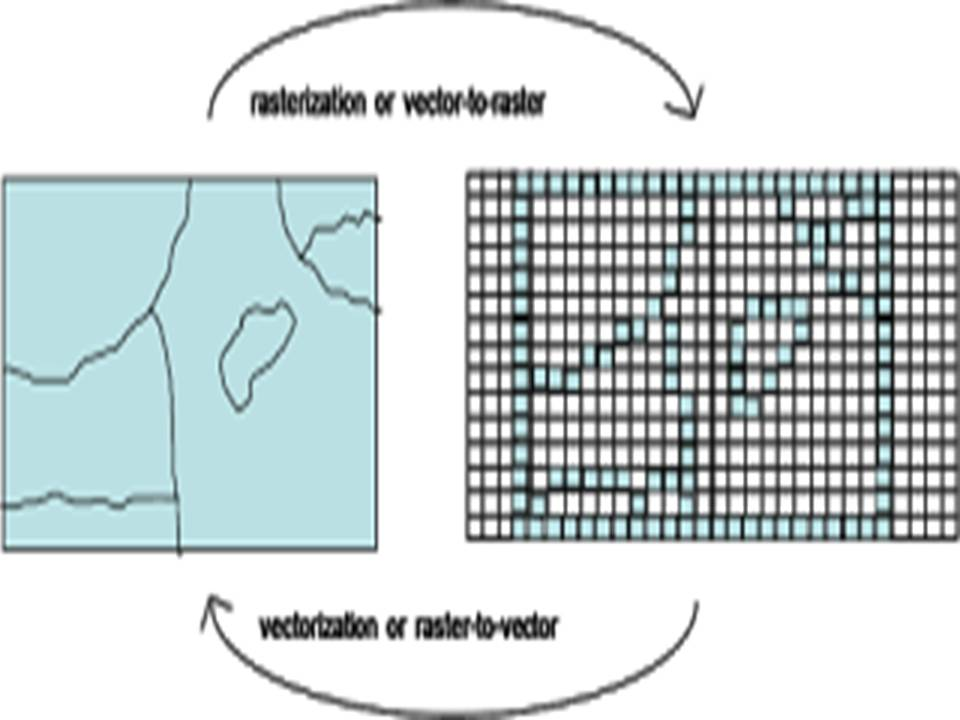
\includegraphics[scale=0.3]{figures/Chapter5AnnisaFathoroni5.jpg}
\caption{Vektorisasi - Annisa Fathoroni}
\label{Vektorisasi - Annisa Fathoroni}
\end{figure}

\end{itemize}

\item Mengapa Dimensi Dari Vektor Dataset Google Bisa Mencapai 300 Dan Ilustrasi Gambar.
\begin{itemize}
\item Penjelasan:

Karena pada masing-masing objek yang terdapat pada dataset akan memiliki identitasnya tersendiri. Apabila dicontohkan dengan penjelasan yang lebih rinci maka dilakukan perumpamaan sederhana. Misalnya untuk sebuah dataset google yang memiliki 3 buah objek yaitu berat, lebar, dan tinggi.  Kemudian dari masing-masing objek tersebut dilakukan perbandingan antara berat dan lebar beserta berat dan tinggi. Hasil yang didapatkan akan memiliki presentasi yang berbeda sehingga dapat diartikan bahwa mesin dapat membedakan objek yang hampir serupa namun tak sama.

\item Ilustrasi Gambar

\begin{figure}[!hbtp]
\centering
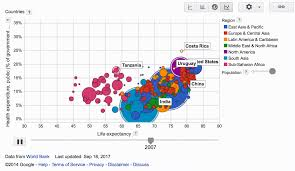
\includegraphics[scale=0.8]{figures/Chapter5AnnisaFathoroni7.jpg}
\caption{Dimensi Vektor Dataset - Annisa Fathoroni}
\label{Dimensi Vektor Dataset - Annisa Fathoroni}
\end{figure}

\end{itemize}

\item Konsep Vektorisasi Untuk Kata Dan Ilustrasi Gambar.
\begin{itemize}
\item  Penjelasan:

Konsep untuk vektorisasi kata sebenarnya sama dengan ketika dilakukan input suatu kata pada mesin pencarian. Kemudian untuk hasilnya akan mengeluarkan ( berupa ) referensi mengenai kata tersebut. Jadi data kata tersebut didapatkan dari hasil pengolahan pada kalimat-kalimat sebelumnya yang telah diolah. Contoh sederhananya pada kalimat berikut ( Please click the alarm icon for more notifications about my channel ), pada kalimat tersebut terdapat konteks yakni channel, kata tersebut akan dijadikan data latih untuk mesin yang akan dipelajari dan diproses. Jadi ketika kita inputkan kta channel, maka mesin akan menampilkan keterkaitannya dengan kata tersebut sehingga akan lebih efisien dan lebih mudah.

\item Ilustrasi Gambar

\begin{figure}[!hbtp]
\centering
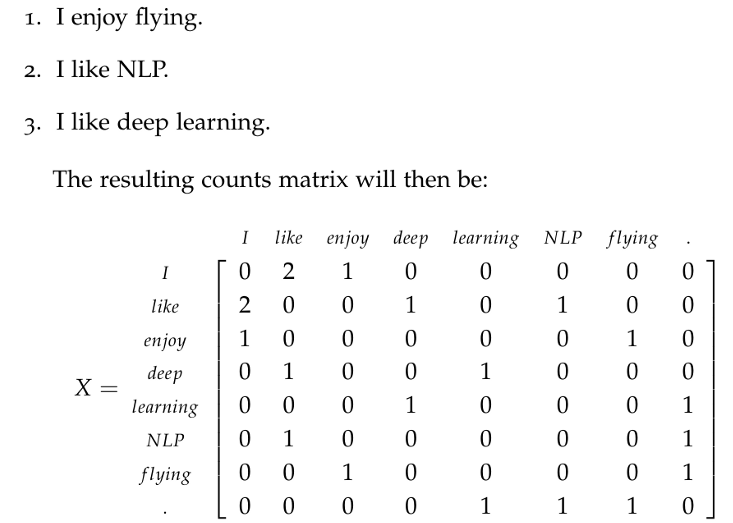
\includegraphics[scale=0.5]{figures/Chapter5AnnisaFathoroni4.png}
\caption{Vektorisasi Untuk Kata - Annisa Fathoroni}
\label{Vektorisasi Untuk Kata - Annisa Fathoroni}
\end{figure}

\end{itemize}

\item Konsep Vektorisasi Untuk Dokumen Dan Ilustrasi Gambar.
\begin{itemize}
\item  Penjelasan:

Untuk vektorisasi dokumen sebenarnya terbilang sama dengan konsep vektorisasi kata, yang membedakan hanya pada proses awalnya ( pada eksekusi awal ). Untuk vektorisasi dokumen ini, mesin akan membaca semua kalimat yang terdapat pada dokumen tersebut, kemudian kalimat yang terdapat pada dokumen tersebut akan di pecah menjadi kata-kata. Seperti itulah konsep vektorisasi dokumen.

\item Ilustrasi Gambar

\begin{figure}[!hbtp]
\centering
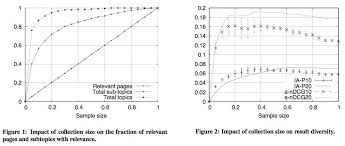
\includegraphics[scale=0.8]{figures/Chapter5AnnisaFathoroni6.jpg}
\caption{Vektorisasi Untuk Dokumen - Annisa Fathoroni}
\label{Vektorisasi Untuk Dokumen - Annisa Fathoroni}
\end{figure}

\end{itemize}

\item Pengertian Mean Dan Standar Devisiasi Beserta Ilustrasi Gambar.
\begin{itemize}
\item  Pengertian Mean:

Mean adalah nilai rata-rata dari beberapa buah data. Nilai mean dapat ditentukan dengan membagi jumlah data dengan banyaknya data. Mean (rata-rata) merupakan suatu ukuran pemusatan data. Mean suatu data juga merupakan statistik karena mampu menggambarkan bahwa data tersebut berada pada kisaran mean data tersebut. Mean tidak dapat digunakan sebagai ukuran pemusatan untuk jenis data nominal dan ordinal.

\item  Pengertian Standar Devisiasi:

Standar Deviasi dan Varians Salah satu teknik statistik yg digunakan untuk menjelaskan homogenitas kelompok. Varians merupakan jumlah kuadrat semua deviasi nilai-nilai individual thd rata-rata kelompok. Sedangkan akar dari varians disebut dengan standar deviasi atau simpangan baku. Standar Deviasi dan Varians Simpangan baku merupakan variasi sebaran data. Semakin kecil nilai sebarannya berarti variasi nilai data makin sama Jika sebarannya bernilai 0, maka nilai semua datanya adalah sama. Semakin besar nilai sebarannya berarti data semakin bervariasi.

\item Ilustrasi Gambar

\begin{figure}[!hbtp]
\centering
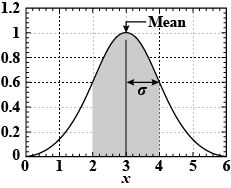
\includegraphics[scale=0.7]{figures/Chapter5AnnisaFathoroni2.png}
\caption{Mean - Annisa Fathoroni}
\label{Mean - Annisa Fathoroni}
\end{figure}

\begin{figure}[!hbtp]
\centering
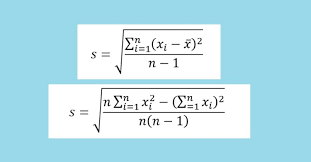
\includegraphics[scale=0.7]{figures/Chapter5AnnisaFathoroni3.png}
\caption{Standar Devisiasi - Annisa Fathoroni}
\label{Standar Devisiasi - Annisa Fathoroni}
\end{figure}

\end{itemize}

\item Penjelasan Skip-gram Dan Ilustrasi Gambar
\begin{itemize}
\item  Penjelasan:

Skip-Gram adalah kebalikannya, yaitu mencoba memprediksi vektor kata-kata yang ada di konteks diberikan vektor kata tertentu. Skip-Gram membuat sepasang kata target dan konteks sebagai sebuah instance sehingga Skip-Gram cenderung lebih baik ketika ukuran corpus sangat besar. 

\item Ilustrasi Gambar

\begin{figure}[!hbtp]
\centering
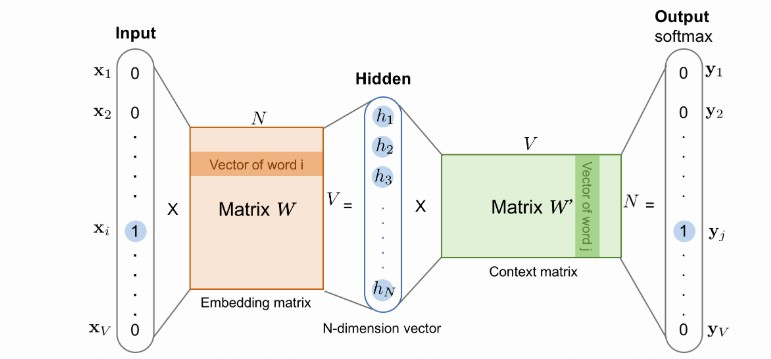
\includegraphics[scale=0.5]{figures/Chapter5AnnisaFathoroni1.jpg}
\caption{Skip Gram - Annisa Fathoroni}
\label{Skip Gram - Annisa Fathoroni}
\end{figure}
\par
\par
\end{itemize}
\par
\par
\end{enumerate}


\section{Tasya Wiendhyra /1164086}
HARI PERTAMA MINGGU KELIMA

\subsection{Kenapa Kata-Kata Harus Di Lakukan Vektorisasi Beserta Ilustrasi}
Karena ketika menggunakan algoritma machine learning tidak bisa  secara langsung menggunakan teks melainkan teks tersebut harus diubah menjadi angka. Kita membutuhkan cara untuk merepresentasikan data teks untuk algoritma pembelajaran mesin, vektorirasi membantu mengubah teks biasa kedalam bentuk vektor yang dapat dimengerti oleh komputer atau machine learning. Kita mungkin ingin melakukan klasifikasi dokumen, sehingga setiap dokumen adalah "input" dan label kelas adalah "output" untuk algoritma prediksinyai. Algoritma mengambil vektor angka sebagai input, oleh karena itu kita perlu mengkonversi dokumen menjadi vektor angka dengan panjang tetap atau sama.
\par Untuk ilustrasinya misal,  saya memiliki kamus berisikan kata-kata {MonkeyLearn, is, not, great}, dan saya ingin membuat vektor teks "MonkeyLearn is great", saya akan memiliki vektor berikut: (1, 1, 0, 0, 1,) .

\subsection{Mengapa Dimensi Dari Vektor Dataset Google Bisa Sampai 300 Beserta Ilustrasi}
Karena di dalam satu dataset berisikan setidaknya 3 Milyar kata dan kalimat. Yang dimana dimensi berisikan kata - kata unik dari data tersebut. Maka dari itu dimensi pada dataset Google bisa mencapai 300.

Untuk ilustrasinya, misalkan kita memiliki sebuah buku dengan tebal 1000 , dimana bukunya dibagi menjadi dua Chapter. Kemudian kita akan menggabungkan kata dari setiap Chapter tersebut. Maka akan didapatkan irisan yang akan berjumlah lebih dari 200. dikarenakan banyak kata yang berbeda beda.

\subsection{Konsep Vektorisasi Untuk Kata}
Konsepnya yaitu kata atau teks akan dihapuskan noisy datanya atau dihapus data yang tidak terpakai, seperti tag html jika ada, titik, koma, dll. Kemudian tokenization artinya kita akan mengelompokan kalimat menjadi token atua membagi kata kata menjadi potingan kecil. Baru setelah itu dilakukan normalisasi untuk mengubah datanya menjadi angka.

Ilustrasinya, misalnya ada beberapa kalimat seperti berikut :
\begin{itemize}
\item There used to be Iron Age.

Kemudian didapatkan token seperti berikut “There”,”was”,”to”,”be”,”used”,”Stone”,”Bronze,”Iron”,”Revolution”,”Digital”,”Age”,”of”,”Now”,”it”,”is”

Maka ketika di cek pada kalimat diatas hasilya seperti berikut 
\item There used to be iron age = [1,0,1,1,1,0,0,1,0,0,1,0,0,0,0]
\end{itemize}

\subsection{Konsep Vektorisasi Untuk Dokumen}
Hampir mirip dengan konsep kata, namun untuk di dokumen biasanya konsepnya digunakan untuk mencari kesamaan atau memprediksi seberapa sering menculan kata dalam 2 kalimat atau 2 paragraf.

Ilustrasinya, misalkan dalam sebuah artikel kita ingin mencari seberapa banyak kata "dimana" muncul. Maka dengan Doc2Vec dapat diprediksi hasilnya.

\subsection{Mean Dan Standar Deviasi}
\subsubsection{Pengertian}
Mean adalah nilai rata-rata dari beberapa buah data. Nilai mean dapat ditentukan dengan membagi jumlah data dengan banyaknya data.

Deviasi standar adalah ukuran ringkasan perbedaan setiap pengamatan dari rata-rata. Deviasi standar mengukur penyebaran data tentang nilai rata-rata. Ini berguna dalam membandingkan set data yang mungkin memiliki mean yang sama tetapi rentang yang berbeda.

\subsubsection{Contoh}
\begin{enumerate}
\item Misalkan kita sudah menghitung tinggi anjing.
\begin{figure}[ht]
\centering
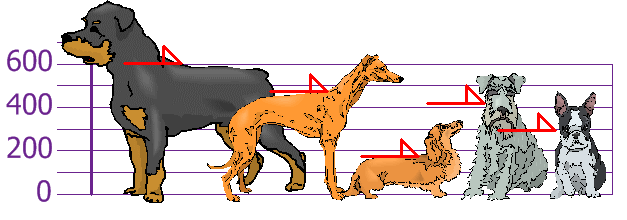
\includegraphics[scale=0.5]{figures/chapter5tasya1.png}
\caption{Contoh Mean dan Standar Deviasi }
\label{Teori}
\end{figure}
\item Tingginya dilihat dari bahu : 600mm, 470mm, 170mm, 430mm and 300mm.
\item Kita hitung mean atau rata ratanya, dengan menjumlahkan seluruh data dan membaginya dengan jumlah n nya hasilnya yaitu 394.
\item Kemudian kita ingin melihat berapa perbedaan tinggi dari anjing - anjing tersebut menggunakan variance. 
\item Baru Gunakan standar deviasi didapatkan hasil 147 mm . DEngan Deviasi Standar kita bisa tahau mana anjing dengan tinggi normal dan anjing yang kekurangan tinggi.
\begin{figure}[ht]
\centering
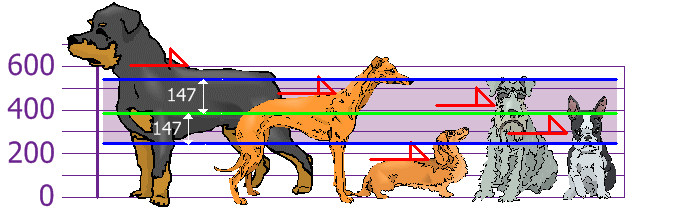
\includegraphics[scale=0.5]{figures/chapter5tasya2.png}
\caption{Contoh Mean dan Standar Deviasi }
\label{Teori}
\end{figure}

\subsection{Skip-gram}
Arsitektur model Skip-gram biasanya  mencoba untuk memprediksi kata konteks sumber (kata-kata sekitarnya) diberi kata target (kata tengah). Contohnya seperti berikut 
\begin{figure}[ht]
\centering
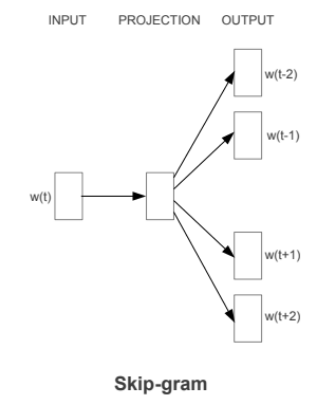
\includegraphics[scale=0.5]{figures/chapter5tasya3.png}
\caption{Contoh Skipgram }
\label{Teori}
\end{figure}
\end{enumerate}


\section{Annisa Cahyani-1164066}
\subsection{Teori}
Penjelasan Tugas Harian 9 ( No 1-6 ). 
\begin{enumerate}
\item Mengapa Kata Harus Di Lakukan Vektorisasi Dan Ilustrasi Gambar
\begin{itemize}
\item Mengapa kata ini harus dilakukan vektorisasi terlebih dahulu karena mesin tersebut hanya mampu atau dapat  membaca data yang berupa angka. Sehingga diperlukannya suatu  vektorisasi kata atau yang bisa disebut dengan mengubah suatu kata menjadi bentuk vektor agar mesin seolah paham apa yang telah kita maksud dan dapat memproses aktifitas atau perintah dengan betul.
\par
\end{itemize}
\par
\par
\item Mengapa Dimensi Dari Vektor Dataset Google Bisa Mencapai 300 Dan Ilustrasi Serta Contoh Gambar
\begin{itemize}
\item Konsep vektorisasi untuk kata yaitu sebuah dimensi dari suatu Vektor Dataset Google yang dapat mencapai 300  dikarenakan pada masing-masing objek yang telah terdapat pada dataset maka akan memiliki suatu identitasnya tersendiri.
\par
\end{itemize}
\par
\par
\item Konsep Vektorisasi Untuk Kata Dan Ilustrasi Gambar
\begin{itemize}
\item Penjelasan tetang vektorisasi untuk kata
\par Vektorisasi Kata adalah suatu hal yang sama dengan pada saat  kita menginputkan suatu kata pada mesin pencari. Kemudian akan  mengeluarkan hasil yang berupa suatu referensi mengenai kata tersebut. Sehingga hasil dari data kata tersebut akan didapatkan dari hasil pengolahan pada kalimat yang telah diolah sebelumnya.
\end{itemize}
\par
\par
\item Konsep Vektorisasi Untuk Dokumen Dan Ilustrasi Gambar
\begin{itemize}
\item Penjelasan tentang vektorisasi untuk dokumen
\par Vektorisasi dokumen yaitu suatu data yang terstruktur karena jauh dari bentuk table baris dan kolom, sehingga Perlu pembentukan data yang terstruktur untuk mewakili dokumen. Maka dari itu kita harus menentukan features yang mewakiliki seluruh kumpulan dokumen.
\end{itemize}
\par
\par
\item Pengertian Mean Dan Standar Devisiasi Beserta Ilustrasi Gambar
\begin{itemize}
\item Penjelasan Mean :
\par Mean yaitu  merupakan suatu nilai rata-rata dari suatu data. Sedangkan mean sendiri juga  dapat dicari dengan menggunakan cara membagi jumlah data dengan banyaknya data, maka dar itulah diperoleh  nilai rata-rata dari suatu data yang dicari.
\par
\item Penjelasan Standar Devisiasi :
\par standar deviasi merupakan sebuah teknik statistik yang diaman digunakan untuk menjelaskan homogenitas kelompok ataupun yang dapat diartikan sebagai nilai statistic. Yang  dimanfaatkan untuk menentukan bagaimana sebaran data pada dalam sampel, serta seberapa dekat dengan  titik data individu ke mean atau  ke rata-rata nilai sampel yang telah ada.
\par
\end{itemize}
\par
\par
\item Penjelasan Skip-gram Dan Ilustrasi Gambar
\begin{itemize}
\item Penjelasan skip-gram
\par Skip-Gram adalah dibutuhkan setiap kata yang ada dalam fokus dan juga mengambil satu-per-satu kata yang ditentukan untuk diberikan setelah pelatihan akan memprediksi probabilitas untuk setiap kata untuk benar-benar muncul di jendela di sekitar kata fokus.
\par
\par
\end{itemize}
\par
\par
\par
\par
\end{enumerate}


\section{PRAKTEK PROGRAM}
\section{Tasya Wiendhyra/1164086}
Praktek Hari Kedua Minggu Kelima
\subsection{Mencoba Dataset}
\subsubsection{Vektor}
\begin{itemize}
\item Pada gambar diatas dapat dilihat bahwa vektor memiliki array sebanyak 300 dimensi. Untuk identitas sektor satu adalah 0.10
\begin{figure}[ht]
\centering
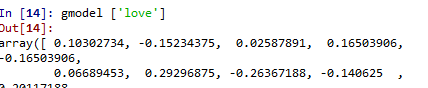
\includegraphics[scale=0.5]{figures/chapter5tasya4.png}
\caption{Vektor Love Tasya}
\label{Praktek}
\end{figure}


\item Pada gambar diatas untuk vektor faith dapat dilihat memliki nilai 0.26 , untuk similaritasnya cukup mendekati vektor love dimana faith dapat dikategorikan dalam satu kategori dengan love.
\begin{figure}[ht]
\centering
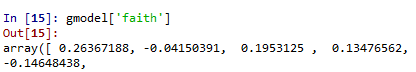
\includegraphics[scale=0.5]{figures/chapter5tasya5.png}
\caption{Vektor Faith Tasya}
\label{Praktek}
\end{figure}


\item Vektor fall hanya memiliki nilai minus yaitu -0.04 , dimana mesin memahami bahwa fall tidak terdapat dalam satu kategori yang sama dengan love dan faith
\begin{figure}[ht]
\centering
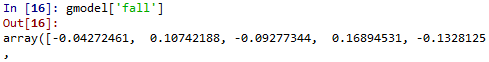
\includegraphics[scale=0.5]{figures/chapter5tasya6.png}
\caption{Vektor Fall Tasya}
\label{Praktek}
\end{figure}


\item  Vektor sick memiliki nilai identitas 1.82 dimana tidak mendekati love, faith maupun fall.
\begin{figure}[ht]
\centering
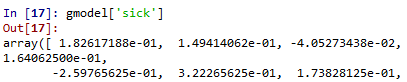
\includegraphics[scale=0.5]{figures/chapter5tasya7.png}
\caption{Vektor Sick Tasya}
\label{Praktek}
\end{figure}


\item Vektor clear memiliki nilai identitas -2,44 dan tidak mendekati nilai dari vektor fall sehingga tidak dapat dijadikan dalam satu kategori
\begin{figure}[ht]
\centering
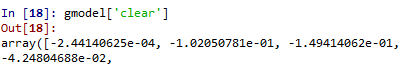
\includegraphics[scale=0.3]{figures/chapter5tasya8.png}
\caption{Vektor Clear Tasya}
\label{Praktek}
\end{figure}

\item Untuk vektor shine -0.12 tidak mendekati vektor manapun.
\begin{figure}[ht]
\centering
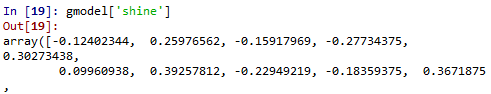
\includegraphics[scale=0.3]{figures/chapter5tasya9.png}
\caption{Vektor Shine Tasya}
\label{Praktek}
\end{figure}


\item Vektor bag memiliki i=nilai identitas -0.03 yang mendekati dengan vektor fall. SEhingga mesin memahami bahwa mungkin saja kedua vektor tersebut berada dalam satu kategori.
\begin{figure}[ht]
\centering
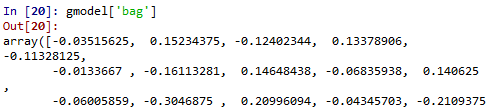
\includegraphics[scale=0.3]{figures/chapter5tasya10.png}
\caption{Vektor Bag Tasya}
\label{Praktek}
\end{figure}


\item Vektor car nilainya 0.13 mendekati vektor love dan faith sehingga mungkin dapat dikategorikan dalam satu kategori.
\begin{figure}[ht]
\centering
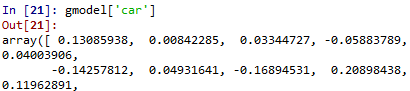
\includegraphics[scale=0.3]{figures/chapter5tasya11.png}
\caption{Vektor Car Tasya}
\label{Praktek}
\end{figure}


\item Vektor wash memiliki nilai 9.46 jauh dari vektor vektor lainnya.
\begin{figure}[ht]
\centering
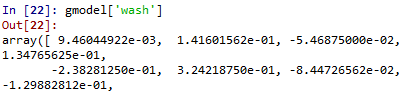
\includegraphics[scale=0.3]{figures/chapter5tasya12.png}
\caption{Vektor Wash Tasya}
\label{Praktek}
\end{figure}


\item Vektor motor memiliki nilai identitas 5.73 yang bisa mendekati vektor wash. Dapat dikatakan bahwa motor dapat dicuci jika diarti dalam satu kategori yang sama.
\begin{figure}[ht]
\centering
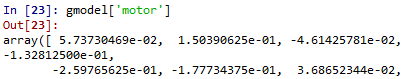
\includegraphics[scale=0.3]{figures/chapter5tasya13.png}
\caption{Vektor Motor Tasya}
\label{Praktek}
\end{figure}
\end{itemize}

\subsubsection{Similariti}
\begin{enumerate}
\item Lihat gambar berikut yang merupakan hasil prediksi similariti
\begin{figure}[ht]
\centering
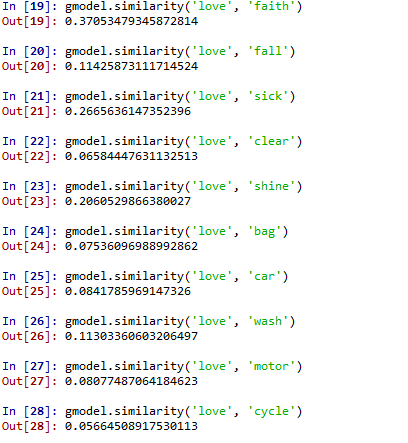
\includegraphics[scale=0.3]{figures/chapter5tasya17.png}
\caption{Similariti Tasya}
\label{Praktek}
\end{figure}

Dapat disimpulkan bahwa
\begin{itemize}
\item Untuk Love dan faith hasilnya adalah 37%
\item Untuk Love dan fall hasilnya adalah 11%
\item Untuk Love dan sick hasilnya adalah 26%
\item Untuk Love dan clear hasilnya adalah 6%
\item Untuk Love dan shine hasilnya adalah 20%
\item Artinya love dan faith memang dalam kategoruiyang sama misalnya dalam kategori percintaan. MEsin sudah mengetahui bahwa keduanya dapat dikategorikan sebagai percintaan.
\end{itemize}
\end{enumerate}

\subsection{Extract Words dan PermuteSentences}
\subsubsection{Extract Words}
ExtractWords merupakan function untuk menambahkan, menghilangkan atau menghapuskan, hal hal yang tidak penting atau tidakperlu di dalam teks. Dalam contoh dibawah ini. menggunakan function extract words untuk menghapus komen dengan python style , mencari data yang diinginkan, dan memberikan spasi pada teks.
\begin{figure}[ht]
\centering
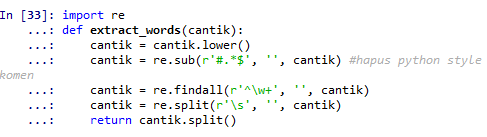
\includegraphics[scale=0.3]{figures/chapter5tasya15.png}
\caption{Extract Words Tasya}
\label{Praktek}
\end{figure}

\subsubsection{PermuteSentences}
PermuteSentences merupakan class yang digunakan unutm melakukan pengocokan secara acak pada data yang ada. Digunakan cara ini agar tidak terjadi kelebihan memori pada saat dijalankan. Contoh dibawah yaitu fungsi akan memanggil lenght. Yang kemudian mendefinisikan variabel req untuk lenght dam melakukan random choice yaitu pengocokan acak untuk kata car.
\begin{figure}[ht]
\centering
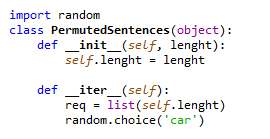
\includegraphics[scale=0.3]{figures/chapter5tasya16.png}
\caption{PermuteSentencesi Tasya}
\label{Praktek}
\end{figure}

\section{Annisa Fathoroni/1164067}
\subsection{Praktek}
Penjelasan Tugas Harian 10 ( No 1-10 ). ( Dan Penanganan Error )
\begin{enumerate}
\item Percobaan Google Dataset ( Perbandingan Dan Similarity ) Untuk Beberapa Data Berikut :
\begin{enumerate}
\item Love

Penjelasan: Pada hasil gambar 'love' dapat dilihat bahwa nilai pada vektor baris pertamanya adalah 0.10302734. Jika dibandingkan dengan gambar 'faith' dapat dikatakan bahwa kedua gambar tersebut tidak dapat dimasukkan pada kategori yang sama.

\begin{figure}[!hbtp]
\centering
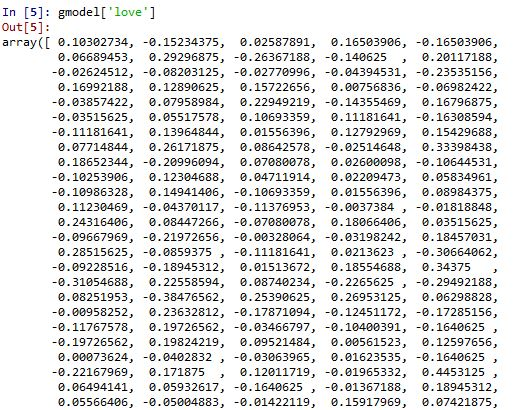
\includegraphics[scale=0.7]{figures/Chapter5AnnisaFathoroni12love.jpg}
\caption{Google Dataset - Annisa Fathoroni, love.}
\label{Google Dataset - Annisa Fathoroni, love.}
\end{figure}

\item Faith

Penjelasan: Pada hasil gambar 'faith' dapat dilihat bahwa nilai pada vektor baris pertamanya adalah 0.26367188. Jika dibandingkan dengan gambar 'fall' dapat dikatakan bahwa kedua gambar tersebut tidak dapat dimasukkan pada kategori yang sama.

\begin{figure}[!hbtp]
\centering
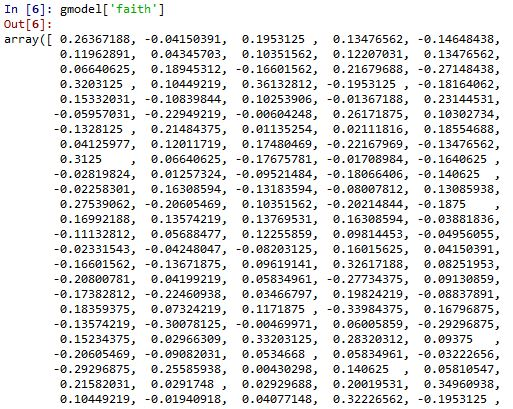
\includegraphics[scale=0.7]{figures/Chapter5AnnisaFathoroni13faith.jpg}
\caption{Google Dataset - Annisa Fathoroni, faith.}
\label{Google Dataset - Annisa Fathoroni, faith.}
\end{figure}

\item Fall

Penjelasan: Pada hasil gambar 'fall' dapat dilihat bahwa nilai pada vektor baris pertamanya adalah -0.04272461. Jika dibandingkan dengan gambar 'sick' dapat dikatakan bahwa kedua gambar tersebut tidak dapat dimasukkan pada kategori yang sama.

\begin{figure}[!hbtp]
\centering
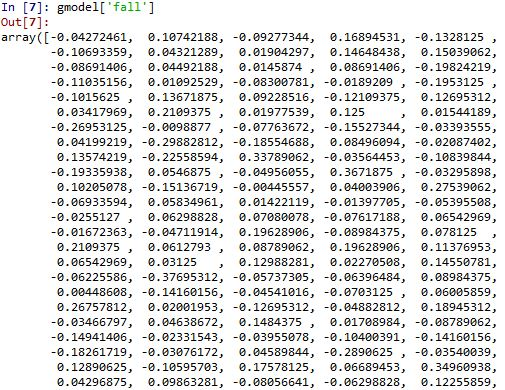
\includegraphics[scale=0.7]{figures/Chapter5AnnisaFathoroni14fall.jpg}
\caption{Google Dataset - Annisa Fathoroni, fall.}
\label{Google Dataset - Annisa Fathoroni, fall.}
\end{figure}

\item Sick

Penjelasan: Pada hasil gambar 'sick' dapat dilihat bahwa nilai pada vektor baris pertamanya adalah 1.82617188e-01. Jika dibandingkan dengan gambar 'clear' dapat dikatakan bahwa kedua gambar tersebut tidak dapat dimasukkan pada kategori yang sama.

\begin{figure}[!hbtp]
\centering
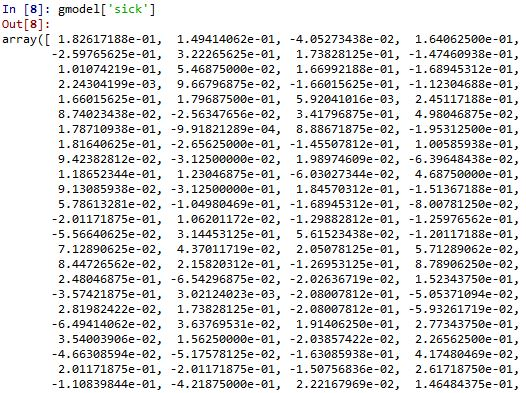
\includegraphics[scale=0.7]{figures/Chapter5AnnisaFathoroni15sick.jpg}
\caption{Google Dataset - Annisa Fathoroni, sick.}
\label{Google Dataset - Annisa Fathoroni, sick.}
\end{figure}

\item Clear

Penjelasan: Pada hasil gambar 'clear' dapat dilihat bahwa nilai pada vektor baris pertamanya adalah -2.44140625e-04. Jika dibandingkan dengan gambar 'shine' dapat dikatakan bahwa kedua gambar tersebut tidak dapat dimasukkan pada kategori yang sama.

\begin{figure}[!hbtp]
\centering
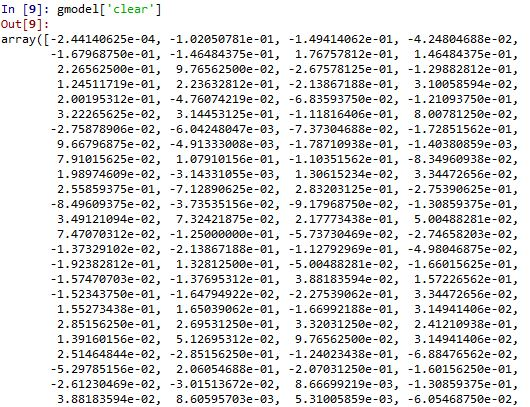
\includegraphics[scale=0.7]{figures/Chapter5AnnisaFathoroni16clear.jpg}
\caption{Google Dataset - Annisa Fathoroni, clear.}
\label{Google Dataset - Annisa Fathoroni, clear.}
\end{figure}

\item Shine

Penjelasan: Pada hasil gambar 'shine' dapat dilihat bahwa nilai pada vektor baris pertamanya adalah -0.12402344. Jika dibandingkan dengan gambar 'bag' dapat dikatakan bahwa kedua gambar tersebut tidak dapat dimasukkan pada kategori yang sama.

\begin{figure}[!hbtp]
\centering
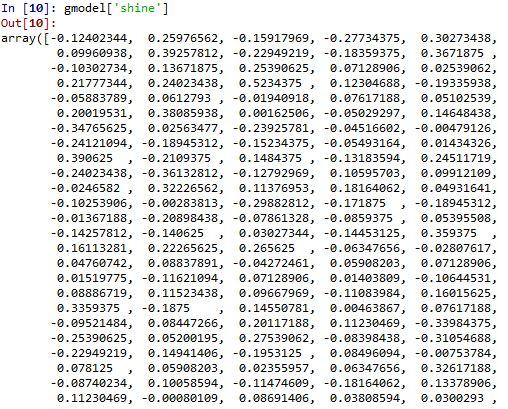
\includegraphics[scale=0.7]{figures/Chapter5AnnisaFathoroni17shine.jpg}
\caption{Google Dataset - Annisa Fathoroni, shine.}
\label{Google Dataset - Annisa Fathoroni, shine.}
\end{figure}

\item Bag

Penjelasan: Pada hasil gambar 'bag' dapat dilihat bahwa nilai pada vektor baris pertamanya adalah -0.03515625. Jika dibandingkan dengan gambar 'car' dapat dikatakan bahwa kedua gambar tersebut tidak dapat dimasukkan pada kategori yang sama.

\begin{figure}[!hbtp]
\centering
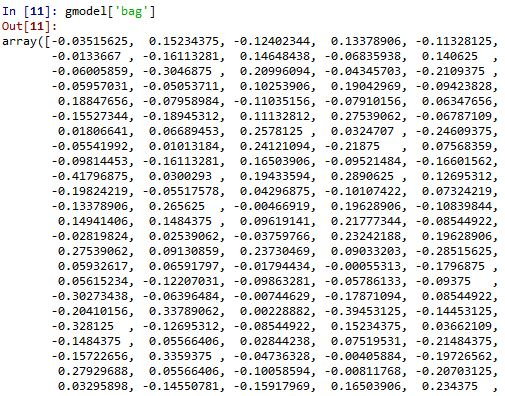
\includegraphics[scale=0.7]{figures/Chapter5AnnisaFathoroni18bag.jpg}
\caption{Google Dataset - Annisa Fathoroni, bag.}
\label{Google Dataset - Annisa Fathoroni, bag.}
\end{figure}

\item Car

Penjelasan: Pada hasil gambar 'car' dapat dilihat bahwa nilai pada vektor baris pertamanya adalah 0.13085938. Jika dibandingkan dengan gambar 'wash' dapat dikatakan bahwa kedua gambar tersebut tidak dapat dimasukkan pada kategori yang sama.

\begin{figure}[!hbtp]
\centering
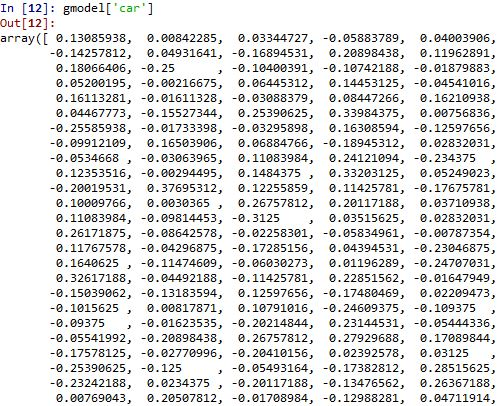
\includegraphics[scale=0.7]{figures/Chapter5AnnisaFathoroni19car.jpg}
\caption{Google Dataset - Annisa Fathoroni, car.}
\label{Google Dataset - Annisa Fathoroni, car.}
\end{figure}

\item Wash

Penjelasan: Pada hasil gambar 'wash' dapat dilihat bahwa nilai pada vektor baris pertamanya adalah 9.46044922e-03. Jika dibandingkan dengan gambar 'motor' dapat dikatakan bahwa kedua gambar tersebut tidak dapat dimasukkan pada kategori yang sama.

\begin{figure}[!hbtp]
\centering
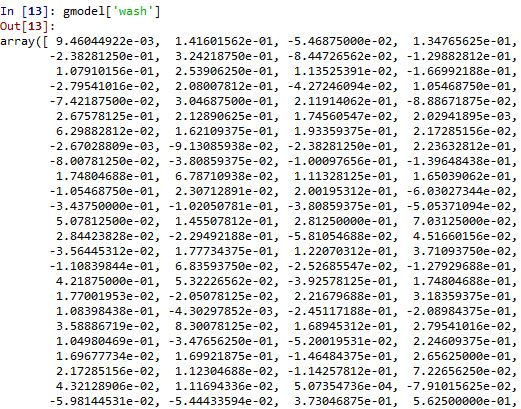
\includegraphics[scale=0.7]{figures/Chapter5AnnisaFathoroni20wash.jpg}
\caption{Google Dataset - Annisa Fathoroni, wash.}
\label{Google Dataset - Annisa Fathoroni, wash.}
\end{figure}

\item Motor

Penjelasan: Pada hasil gambar 'motor' dapat dilihat bahwa nilai pada vektor baris pertamanya adalah 5.73730469e-02. Jika dibandingkan dengan gambar 'cycle' dapat dikatakan bahwa kedua gambar tersebut tidak dapat dimasukkan pada kategori yang sama.

\begin{figure}[!hbtp]
\centering
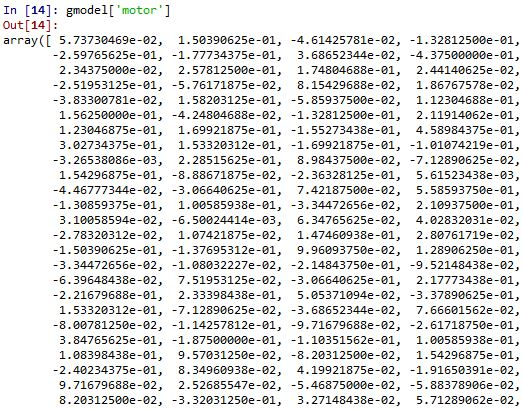
\includegraphics[scale=0.7]{figures/Chapter5AnnisaFathoroni21motor.jpg}
\caption{Google Dataset - Annisa Fathoroni, motor.}
\label{Google Dataset - Annisa Fathoroni, motor.}
\end{figure}

\item Cycle

Penjelasan: Pada hasil gambar 'cycle' dapat dilihat bahwa nilai pada vektor baris pertamanya adalah 0.04541016. Jika dibandingkan dengan gambar 'love' dapat dikatakan bahwa kedua gambar tersebut tidak dapat dimasukkan pada kategori yang sama.

\begin{figure}[!hbtp]
\centering
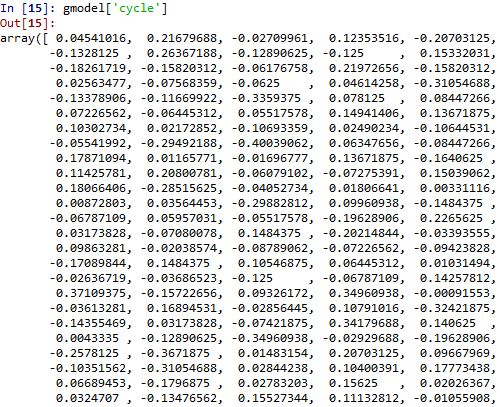
\includegraphics[scale=0.7]{figures/Chapter5AnnisaFathoroni22cycle.jpg}
\caption{Google Dataset - Annisa Fathoroni, cycle.}
\label{Google Dataset - Annisa Fathoroni, cycle.}
\end{figure}

\item Similarity

Penjelasan: Pada hasil gambar 'car' dapat dilihat bahwa nilai pada vektor baris pertamanya adalah 0.13085938. Jika dibandingkan dengan gambar 'love', 'sick', 'clear', 'motor', 'wash' dapat dikatakan bahwa semua gambar tersebut yang paling mendekati adalah 'sick'.

\begin{figure}[!hbtp]
\centering
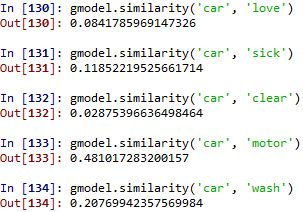
\includegraphics[scale=0.7]{figures/Chapter5AnnisaFathoroni23.jpg}
\caption{Google Dataset - Annisa Fathoroni, similarity.}
\label{Google Dataset - Annisa Fathoroni, similarity.}
\end{figure}

\end{enumerate}

\item Penjelasan Dan Ilustrasi ExtractWords Dan PermuteSentences
\begin{itemize}

\begin{figure}[!hbtp]
\centering
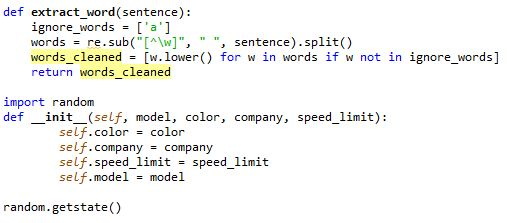
\includegraphics[scale=0.7]{figures/Chapter5AnnisaFathoroni32.jpg}
\caption{Extract Word dan PermuteSentences - Annisa Fathoroni}
\label{Extract Word dan PermuteSentences - Annisa Fathoroni}
\end{figure}

\item ExtractWords

Penjelasan:  Pada kalimat 'This isn't really a sentence' yang  akan dipisahkan perkata. Dimana library re dan library string di import terlebih dahulu. Lalu variable out mendefinisikan X untuk mengembalikan string pada objek line yang telah di split. Kemudian, X dikembalikan berdasarkan jumlah kata.

\begin{figure}[!hbtp]
\centering
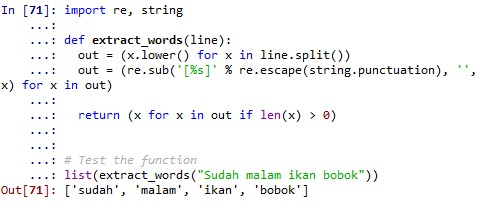
\includegraphics[scale=0.7]{figures/Chapter5AnnisaFathoroni29.jpeg}
\caption{ExtractWord - Annisa Fathoroni}
\label{ExtractWord - Annisa Fathoroni}
\end{figure}

\item PermuteSentences

Penjelasan: Digunakan untuk melakukan pengocokan atau acak pada text yang diiginkan.

\begin{figure}[!hbtp]
\centering
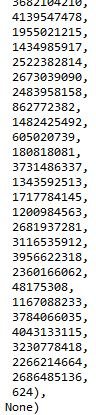
\includegraphics[scale=0.7]{figures/Chapter5AnnisaFathoroni31.jpg}
\caption{PermuteSentences - Annisa Fathoroni}
\label{PermuteSentences - Annisa Fathoroni}
\end{figure}

\end{itemize}
\end{enumerate}


\section{Annisa Cahyani-1164066}
\subsection{Praktek}
Penjelasan Tugas Harian 10  
\begin{enumerate}
\item Percobaan Google Dataset ( Perbandingan Dan Similarity ) Untuk Beberapa DataSebagai  Berikut :
\begin{enumerate}
\item Love :
\par Penjelasannya  pada gambar love disini menghasilkan 0.10  berdasarkan hasil dari awalan nilai tersebut berasal dari dataset sebagai perbandingan yang awal.
\par
\begin{figure}[!hbtp]
\centering
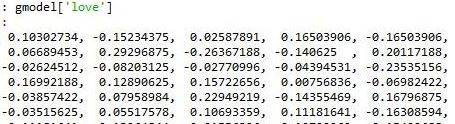
\includegraphics[scale=0.2]{figures/cahya-love.jpg}
\caption{cahya-love}
\label{cahya-love}
\end{figure}
\par
\item Faith : 
\par pada gambar faith menghasilkan nilai yaitu 0.26 berdasarkan dari hasil nilai awal dari dataset yaitu sebagai perbandingan awal.
\par
\begin{figure}[!hbtp]
\centering
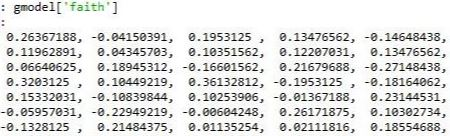
\includegraphics[scale=0.2]{figures/cahya-faith.jpg}
\caption{ cahya-faith}
\label{ cahya-faith}
\end{figure}
\par
\item Fall :  
\par Pada gambar bagian fall disini menghasilkan nilai -0.04 nilai ini  berdasarkan hasil dari dataset  sebgai perbandingan awal
\par
\begin{figure}[!hbtp]
\centering
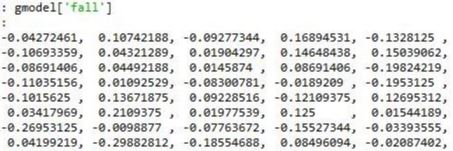
\includegraphics[scale=0.2]{figures/cahya-fall.jpg}
\caption{ cahya - fall}
\label{cahya - fall}
\end{figure}
\par
\item Sick :
\par Penjelasan pada gambar sick yaitu menghasilkan nilai 1.82 yang dimana nilai ini berdasarkan dari dataset sebagai perbandingan awal.
\par
\begin{figure}[!hbtp]
\centering
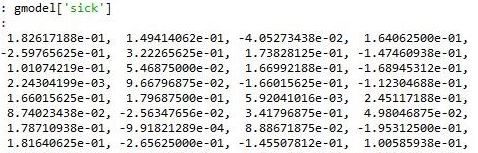
\includegraphics[scale=0.2]{figures/cahya-sick.jpg}
\caption{ cahya - sick}
\label{cahya - sick}
\end{figure}
\par
\item Clear :
\par Pada gambar clear disini menghasilkan nilai -2.44  yaitu sebagai nilai berdasarkan dari dataset sebagai perbandingan awal.
\par
\begin{figure}[!hbtp]
\centering
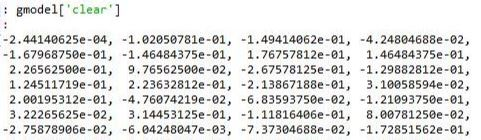
\includegraphics[scale=0.2]{figures/cahya-clear.jpg}
\caption{ cahya - clear}
\label{cahya - clear}
\end{figure}
\par
\item Shine : 
\par Penjelasan pada gambar shine ini menghasilkan nilai -0.12 yaitu berdasarkan dari dataset sebagai perbandingan awal.
\par
\begin{figure}[!hbtp]
\centering
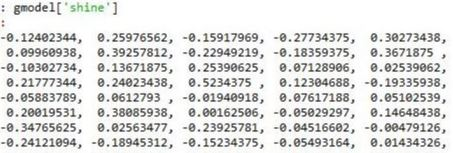
\includegraphics[scale=0.2]{figures/cahya-shine.jpg}
\caption{cahya - shine}
\label{ cahya - shine }
\end{figure}
\par
\item Bag :  
\par Pada gambar bag disini menghasilkan nilai -0.03 yang dimana berdasarkan dari dataset sebagai untuk perbandingan awal.
\par
\begin{figure}[!hbtp]
\centering
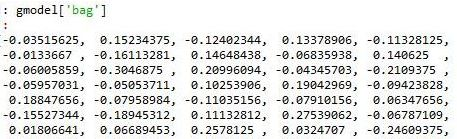
\includegraphics[scale=0.2]{figures/cahya-bag.jpg}
\caption{ cahya - bag}
\label{cahya - bag}
\end{figure}
\par
\item Car :  
\par Penjelasan gambar bagian car menghasilakan nilai 0.13  yang dimanai nilai tersebeut berdasarkan dari dataset untuk perbandingan awal 
\par
\begin{figure}[!hbtp]
\centering
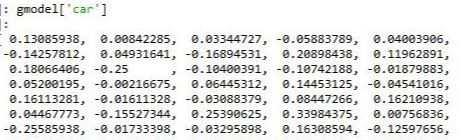
\includegraphics[scale=0.2]{figures/cahya-car.jpg}
\caption{cahya - car}
\label{ cahya - car}
\end{figure}
\par
\item Wash :  
\par Pada gambar wash menghasilkan nilai 9.46 yaitu nilai tersebut berdasarkan dari dataset sebagai perbandingan awal
\par
\begin{figure}[!hbtp]
\centering
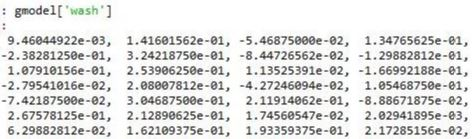
\includegraphics[scale=0.2]{figures/cahya-wash.jpg}
\caption{cahya - wash}
\label{ cahya - wash}
\end{figure}
\par
\item Motor :  
\par Penjelasan pada gambar motor  menghasilkan nilai 5.73  nilai ini  berdasarkan dari dataset sebagai perbandingan awal
\par
\begin{figure}[!hbtp]
\centering
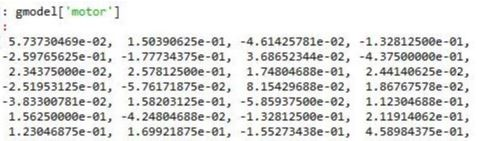
\includegraphics[scale=0.2]{figures/cahya-motor.jpg}
\caption{ cahya - motor}
\label{cahya - motor}
\end{figure}
\par
\item Cycle :  
\par Pada gambar cycle disini menghasilkan nilai 0.04 nilai ini berdasarkan dari dataset sebagai perbandingan awal
\par
\begin{figure}[!hbtp]
\centering
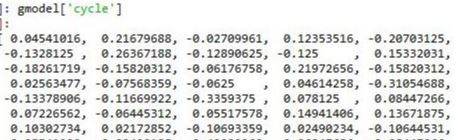
\includegraphics[scale=0.2]{figures/cahya-cycle.jpg}
\caption{cahya - cycle}
\label{cahya - caycle}
\end{figure}
\par
\item Similarity :
\par  Perbandingan antara beberapa dataset yang telah diuji untuk dibandingkan. Untuk contohnya seperti pada gambar dibawah. Nilai Yang paling besar dapat menentukan bahwa kedua dataset tersebut bisa dikategorikan sama ( atau bisa dikelompokkan ).
\par
\begin{figure}[!hbtp]
\centering
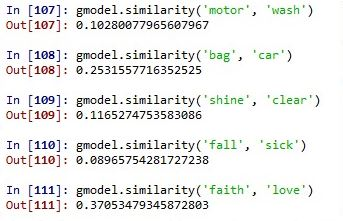
\includegraphics[scale=0.2]{figures/cahya-similarity.jpg}
\caption{Cahya - Similarity}
\label{Cahya - Similarity}
\end{figure}
\par
\end{enumerate}
\par
\par
\par
\par
\item Penjelasan Dan Ilustrasi Extract\_Words Dan PermuteSentences
\begin{itemize}
\item Extract\_Words :
\par Penjelasan : extract  word itu berfungsi untuk memecahkan suatu katautnuk  menjadi beberapa komponen atau yang lebih mudahnya itu  kata yang dieksekusidan  dipecah kemudian dikelompokkan lagi sesuai dengan keinginan. 
\par Kemudian dari seusai hasil yang didaptkan untuk contoh ini itu terdapat satu kalimat untuk yang terbentuk dari 6 kata. kemudian pada  kata tersebut akan di pisahkan menggunakansuatu  perintah kemudian hasinya akan keluar.
\par
\begin{figure}[!hbtp]
\centering
\includegraphics[scale=0.2]{figures/cahya-exract-word.jpg}
\caption{cahya-extract-word}
\label{cahya-extraxt-word}
\end{figure}
\par
\par
\item PermuteSentences 
\par PermuteSentences itu  digunakan untuk melakukan suatu pengocokan atau random pada text yang diiginkan.
\par pada gambar  mengeluarkan sebuah hasi yang dimana telah berupa pengacakan, pengocokan kata, huruf atau kalimat yang telah didefinisikan pada perintah untuk dieksekusi. 
\par
\par
\begin{figure}[!hbtp]
\centering
\includegraphics[scale=0.2]{figures/cahya-permute.jpg}
\caption{cahya - permute}
\label{cahya - permute}
\end{figure}
\par
\par
\end{itemize}
\end{enumerate}